% ============================================================
%  CS3401 – Chapter 7: Greedy Algorithms  (NEW chapter)
% ============================================================
\documentclass[aspectratio=169]{beamer}
% ============================================================
%  CS3401 – Algorithm Design and Analysis
%  Shared Beamer Theme (input this file in every chapter)
%  Prince Sattam Bin Abdulaziz University – CCES
% ============================================================

% ---------- PACKAGES ----------------------------------------
\usepackage[utf8]{inputenc}
\usepackage[T1]{fontenc}
\usepackage{lmodern}
\usepackage{amsmath,amssymb,amsthm}
\usepackage{tikz}
\usepackage{pgfplots}
\usepackage{booktabs}
\usepackage{xcolor}
\usepackage{graphicx}
\usepackage{listings}
\usepackage[normalem]{ulem}
\usepackage{algorithm}
\usepackage{algpseudocode}
\usepackage{multicol}
\usepackage{array}
\usepackage{colortbl}
\usepackage{tabularx}
\usepackage{makecell}

\usetikzlibrary{
  arrows.meta, shapes.geometric, shapes.symbols,
  positioning, calc, fit, backgrounds,
  decorations.pathreplacing, decorations.markings,
  matrix, chains, trees
}
\pgfplotsset{compat=1.18}

% ---------- COLOR PALETTE -----------------------------------
\definecolor{PrimaryDark}{RGB}{10,72,92}
\definecolor{PrimaryMid}{RGB}{18,114,145}
\definecolor{PrimaryLight}{RGB}{185,224,238}
\definecolor{AccentOrange}{RGB}{210,103,22}
\definecolor{AccentYellow}{RGB}{252,198,40}
\definecolor{SuccessGreen}{RGB}{32,122,66}
\definecolor{AlertRed}{RGB}{172,46,46}
\definecolor{CodeBg}{RGB}{244,246,250}
\definecolor{DarkText}{RGB}{28,32,40}
\definecolor{LightRule}{RGB}{210,225,232}
\tikzset{processstep/.style={draw=PrimaryMid, fill=PrimaryLight!35, rounded corners=2pt,
  align=center, minimum width=4.2cm, minimum height=0.55cm, font=\small}}

% ---------- BEAMER SETTINGS ---------------------------------
\setbeamertemplate{navigation symbols}{}
\setbeamertemplate{caption}[numbered]

% Fonts
\setbeamerfont{normal text}{size=\small}
\setbeamerfont{title}{series=\bfseries,size=\LARGE}
\setbeamerfont{subtitle}{series=\normalfont,size=\large}
\setbeamerfont{frametitle}{series=\bfseries,size=\large}
\setbeamerfont{framesubtitle}{series=\normalfont,size=\small}
\setbeamerfont{block title}{series=\bfseries,size=\normalsize}
\setbeamerfont{footline}{size=\tiny}
\addtobeamertemplate{frame begin}{\small\enlargethispage{1cm}}{}
\setlength{\tabcolsep}{2pt}

% Colors
\setbeamercolor{normal text}{fg=DarkText,bg=white}
\setbeamercolor{frametitle}{bg=PrimaryDark,fg=white}
\setbeamercolor{title}{fg=white}
\setbeamercolor{subtitle}{fg=PrimaryLight}
\setbeamercolor{author}{fg=white}
\setbeamercolor{date}{fg=PrimaryLight}
\setbeamercolor{institute}{fg=PrimaryLight}
\setbeamercolor{block title}{bg=PrimaryMid,fg=white}
\setbeamercolor{block body}{bg=PrimaryLight!35,fg=DarkText}
\setbeamercolor{block title alerted}{bg=AlertRed,fg=white}
\setbeamercolor{block body alerted}{bg=AlertRed!12,fg=DarkText}
\setbeamercolor{block title example}{bg=SuccessGreen,fg=white}
\setbeamercolor{block body example}{bg=SuccessGreen!12,fg=DarkText}
\setbeamercolor{itemize item}{fg=PrimaryMid}
\setbeamercolor{itemize subitem}{fg=AccentOrange}
\setbeamercolor{enumerate item}{fg=PrimaryMid}
\setbeamercolor{enumerate subitem}{fg=AccentOrange}
\setbeamercolor{alerted text}{fg=AlertRed}
\setbeamercolor{structure}{fg=PrimaryMid}
\setbeamercolor{section in toc}{fg=PrimaryDark}
\setbeamercolor{section in toc shaded}{fg=PrimaryDark}
% override Beamer's transparency-based shading so TOC entries stay fully visible
\setbeamertemplate{section in toc shaded}{\inserttocsection\par}
\setbeamercolor{subsection in toc}{fg=PrimaryMid}
\setbeamercolor{footer rule}{bg=LightRule}

% Item symbols
\setbeamertemplate{itemize item}{%
  \scriptsize\raise1.5pt\hbox{\color{PrimaryMid}$\blacktriangleright$}}
\setbeamertemplate{itemize subitem}{%
  \scriptsize\raise1pt\hbox{\color{AccentOrange}$\bullet$}}
\setbeamertemplate{itemize subsubitem}{%
  \scriptsize\raise1pt\hbox{\color{PrimaryDark}$\circ$}}
\setbeamertemplate{enumerate item}{%
  \color{PrimaryMid}\textbf{\insertenumlabel.}}

% Frame title
\makeatletter
\setbeamertemplate{frametitle}{%
  \nointerlineskip
  \begin{beamercolorbox}[wd=\paperwidth,ht=2.4em,dp=0.9em,%
                         leftskip=1.2em,rightskip=1.2em]{frametitle}
    \usebeamerfont{frametitle}\insertframetitle\strut
    \ifx\insertframesubtitle\@empty\else
      \hspace{0.6em}\textcolor{PrimaryLight!80}{\footnotesize|}\hspace{0.4em}%
      {\usebeamerfont{framesubtitle}\textcolor{PrimaryLight}\insertframesubtitle}%
    \fi
  \end{beamercolorbox}
  \nointerlineskip
  \begin{beamercolorbox}[wd=\paperwidth,ht=0.3pt,dp=0pt]{structure}
  \end{beamercolorbox}
}
\makeatother

% Footer
\setbeamertemplate{footline}{%
  \begin{beamercolorbox}[wd=\paperwidth,ht=0.4pt,dp=0pt]{footer rule}{}
  \end{beamercolorbox}
  \leavevmode
  \hbox{%
    \begin{beamercolorbox}[wd=0.60\paperwidth,ht=1.8em,dp=0.6em,leftskip=1em]{normal text}%
      \textcolor{PrimaryDark}{\tiny\textbf{CS3401} \textendash{} Algorithm Design \& Analysis%
        \quad\textbar\quad CCES, PSAU}%
    \end{beamercolorbox}%
    \begin{beamercolorbox}[wd=0.40\paperwidth,ht=1.8em,dp=0.6em,rightskip=1em,right]{normal text}%
      \textcolor{PrimaryDark}{\tiny\insertshorttitle%
        \quad\textbar\quad\insertframenumber\,/\,\inserttotalframenumber}%
    \end{beamercolorbox}%
  }%
}

% Title page
\setbeamertemplate{title page}{%
  
\begin{tikzpicture}[remember picture,overlay]
    \fill[PrimaryDark](current page.north west) rectangle (current page.south east);
    \fill[PrimaryMid,opacity=0.45]
      ([shift={(2.5cm,-2.5cm)}]current page.north east) circle(5.5cm);
    \fill[AccentOrange,opacity=0.10]
      ([shift={(-1.5cm,2.0cm)}]current page.south west) circle(4.2cm);
    \draw[white,opacity=0.08,line width=40pt]
      ([shift={(0cm,-0.5cm)}]current page.north west)
      to[out=-30,in=210]
      ([shift={(0cm,0.5cm)}]current page.south east);
  \end{tikzpicture}%
  \vspace{0.7cm}
  \begin{center}
    {\tiny\textcolor{PrimaryLight}{\textbf{CCES} \textendash{}
      College of Computer Engineering and Sciences}}\\[0.2em]
    {\tiny\textcolor{PrimaryLight}{Prince Sattam Bin Abdulaziz University}}\\[1.2em]
    {\footnotesize\textcolor{AccentYellow}{\textbf{CS3401 \textendash{} Algorithm Design and Analysis}}}\\[1.5em]
    \textcolor{PrimaryMid}{\rule{0.55\textwidth}{0.6pt}}\\[0.9em]
    {\Large\usebeamerfont{title}\textcolor{white}{\inserttitle}}\\[0.4em]
    {\small\usebeamerfont{subtitle}\textcolor{PrimaryLight}{\insertsubtitle}}\\[0.7em]
    \textcolor{PrimaryMid}{\rule{0.55\textwidth}{0.6pt}}\\[1.2em]
    {\footnotesize\textcolor{PrimaryLight}{\insertdate}}\\[0.6em]
    % Instructors row
    \begin{tikzpicture}[baseline=(current bounding box.center)]
      % Dr. Khalil – rounded photo
      \begin{scope}
        \clip (-3.2,0) circle (0.58cm);
        \node at (-3.2,0)
          {
\includegraphics[width=1.16cm,height=1.16cm,keepaspectratio=false]{khalil}};
      \end{scope}
      \draw[white,line width=0.9pt] (-3.2,0) circle (0.58cm);
      \node[text=white,font=\scriptsize\bfseries,anchor=west] at (-2.54,0)
        {Dr.\ Khalil Chebil};
      % Dr. Esraa – placeholder circle
      \draw[white,line width=0.9pt] (1.2,0) circle (0.58cm);
      \node[text=PrimaryLight,font=\normalsize\bfseries] at (1.2,0) {E};
      \node[text=white,font=\scriptsize\bfseries,anchor=west] at (1.86,0)
        {Dr.\ Esraa};
    \end{tikzpicture}
  \end{center}%
}

% Auto section-divider slide — background set via Beamer color system for reliability
\AtBeginSection[]{%
  {%
    \setbeamercolor{background canvas}{bg=PrimaryDark}%
    \begin{frame}[plain,noframenumbering]
      \begin{tikzpicture}[remember picture,overlay]
        \fill[PrimaryMid,opacity=0.35]
          ([shift={(0cm,-1.5cm)}]current page.north) circle(6.5cm);
        \node[text=white,opacity=0.06,font=\fontsize{120}{120}\bfseries]
          at ([shift={(-1cm,0cm)}]current page.center)
          {\insertsectionnumber};
      \end{tikzpicture}
      \vfill
      \begin{center}
        {\large\textcolor{AccentYellow}{\textbf{Section \insertsectionnumber}}}\\[0.6em]
        {\LARGE\textcolor{white}{\textbf{\insertsectionhead}}}
      \end{center}
      \vfill
    \end{frame}
  }%
}

% ---------- LISTINGS STYLE ----------------------------------
\lstset{
  basicstyle=\ttfamily\footnotesize,
  backgroundcolor=\color{CodeBg},
  keywordstyle=\color{PrimaryMid}\bfseries,
  commentstyle=\color{SuccessGreen}\itshape,
  stringstyle=\color{AccentOrange},
  numberstyle=\tiny\color{gray!70},
  frame=tb,
  framerule=0.5pt,
  rulecolor=\color{PrimaryLight},
  numbers=left,
  numbersep=6pt,
  showstringspaces=false,
  breaklines=true,
  tabsize=2,
  xleftmargin=1.8em,
  framexleftmargin=1.8em,
  captionpos=b,
  language=Java,
  morekeywords={var,let,const}
}

% ---------- PSEUDOCODE STYLE --------------------------------
\algrenewcommand\algorithmicprocedure{\textbf{Algorithm}}
\algrenewcommand\algorithmicfunction{\textbf{Function}}
\algrenewcommand\algorithmicif{\textbf{if}}
\algrenewcommand\algorithmicelse{\textbf{else}}
\algrenewcommand\algorithmicthen{\textbf{then}}
\algrenewcommand\algorithmicwhile{\textbf{while}}
\algrenewcommand\algorithmicfor{\textbf{for}}
\algrenewcommand\algorithmicforall{\textbf{for all}}
\algrenewcommand\algorithmicreturn{\textbf{return}}
\algrenewcommand\algorithmicend{\textbf{end}}
\algrenewcommand\algorithmicdo{}
\algrenewcommand\algorithmicrequire{\textbf{Input:}}
\algrenewcommand\algorithmicensure{\textbf{Output:}}

% ---------- CUSTOM COMMANDS ---------------------------------
\newcommand{\bigO}[1]{$\mathcal{O}(#1)$}
\newcommand{\bigTheta}[1]{$\Theta(#1)$}
\newcommand{\bigOmega}[1]{$\Omega(#1)$}
\newcommand{\highlight}[1]{\colorbox{AccentYellow!55}{\strut #1}}
\newcommand{\important}[1]{\textcolor{AlertRed}{\bfseries #1}}
\newcommand{\keyword}[1]{\textcolor{PrimaryMid}{\bfseries #1}}
\newcommand{\concept}[1]{\textcolor{AccentOrange}{\bfseries #1}}

% Colored table column types
\newcolumntype{H}{>{\columncolor{PrimaryDark}\color{white}\bfseries\centering\arraybackslash}m{2.5cm}}
\newcolumntype{Z}{>{\columncolor{PrimaryLight!40}\centering\arraybackslash}m{2cm}}

% Reference boxes
\newcommand{\refbox}[1]{%
  \begin{beamercolorbox}[rounded=true,shadow=false,leftskip=0.5em,rightskip=0.5em,%
                          ht=1.6em,dp=0.5em]{block title}
    \small\textit{Reference:} #1
  \end{beamercolorbox}%
}

% Inline complexity tag
\newcommand{\ctag}[1]{%
  \hfill\tikz[baseline]{\node[fill=AlertRed,text=white,rounded corners=2pt,
    font=\bfseries\scriptsize,inner sep=2pt,outer sep=0pt]{$\mathcal{O}(#1)$};}%
}


\title[Ch.\,7 -- Greedy Algorithms]{Chapter 7}
\subtitle{Greedy Algorithms}
\date{Academic Year 2026\,--\,2027}

\begin{document}

\begin{frame}[plain]\titlepage\end{frame}
\begin{frame}{Chapter Overview}
  \begin{center}
    \begin{minipage}{0.85\textwidth}
      \tableofcontents[hideallsubsections,sectionstyle=show/shaded]
    \end{minipage}
  \end{center}
\end{frame}

% ============================================================
\section{Introduction to Greedy Algorithms}
% ============================================================

\begin{frame}[shrink=12]{What is a Greedy Algorithm?}
  \begin{block}{Definition}
    A \keyword{greedy algorithm} builds a solution step by step,
    always making the \emph{locally optimal choice} (the one that looks
    best at the current moment), without reconsidering past decisions.
  \end{block}
  \vspace{0.4em}
  \begin{columns}[T]
    \column{0.50\textwidth}
      \textbf{Greedy vs.\ Dynamic Programming:}
      \begin{tabular}{lll}
        \toprule
        & \textbf{Greedy} & \textbf{DP} \\
        \midrule
        Sub-problems & independent & overlapping \\
        Choices & one per step & all options \\
        Speed & fast (usually $\mathcal{O}(n\log n)$) & slower \\
        Correctness & not always! & always correct \\
        \bottomrule
      \end{tabular}
    \column{0.45\textwidth}
      \begin{alertblock}{Greedy is not always correct}
        The change-making problem with coins $\{1,3,4\}$ and target 6:
        \begin{itemize}
          \item Greedy: $4+1+1 = 3$ coins ← \alert{suboptimal}
          \item DP: $3+3 = 2$ coins ← optimal
        \end{itemize}
      \end{alertblock}
      \begin{exampleblock}{When greedy works}
        When the problem has \emph{greedy choice property}:
        a globally optimal solution includes the locally optimal choice.
      \end{exampleblock}
  \end{columns}
\end{frame}

% ============================================================
\section{Activity Selection Problem}
% ============================================================

\begin{frame}[shrink=25]{Activity Selection}
  \begin{block}{Problem}
    Given $n$ activities each with start time $s_i$ and finish time $f_i$,
    select the maximum number of \emph{non-overlapping} activities.
  \end{block}
  \vspace{0.3em}
  \begin{columns}[T]
    \column{0.55\textwidth}
      \textbf{Greedy strategy:} Always pick the activity with the
      \emph{earliest finish time} that does not conflict with the
      previously selected activity.

      \vspace{0.3em}
      \textbf{Algorithm:}
      \begin{algorithmic}[1]
        \State Sort activities by finish time
        \State Select activity 1 (earliest finish)
        \State $\text{last} \gets 1$
        \For{$i \gets 2$ \textbf{to} $n$}
          \If{$s_i \geq f_{\text{last}}$}
            \State Select activity $i$;\; $\text{last} \gets i$
          \EndIf
        \EndFor
      \end{algorithmic}
      Complexity: $\mathcal{O}(n\log n)$ (sort) + $\mathcal{O}(n)$ (scan)
    \column{0.40\textwidth}
      \textbf{Example:}
      \vspace{0.2em}

      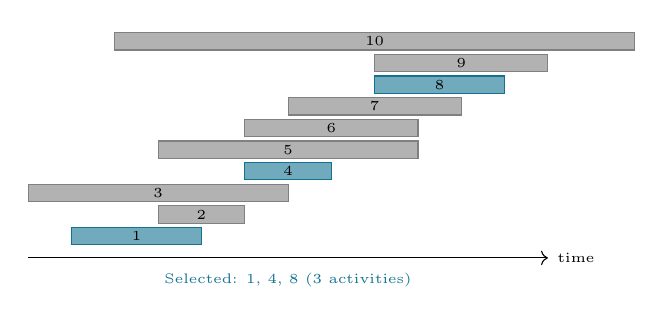
\begin{tikzpicture}[scale=0.55]
        \draw[->] (0,0) -- (12,0) node[right,font=\tiny]{time};
        \foreach \i/\s/\f/\c in
          {1/1/4/PrimaryMid, 2/3/5/gray, 3/0/6/gray,
           4/5/7/PrimaryMid, 5/3/9/gray, 6/5/9/gray,
           7/6/10/gray, 8/8/11/PrimaryMid, 9/8/12/gray, 10/2/14/gray}
        {
          \fill[\c!60] (\s,\i*0.5-0.2) rectangle (\f,\i*0.5+0.2);
          \draw[\c] (\s,\i*0.5-0.2) rectangle (\f,\i*0.5+0.2);
          \node[font=\tiny] at ({(\s+\f)/2},\i*0.5) {\i};
        }
        \node[font=\tiny,text=PrimaryMid] at (6,-0.5)
          {Selected: 1, 4, 8 (3 activities)};
      \end{tikzpicture}
      \vspace{0.3em}
      \textbf{Proof of correctness:} Exchange argument — replacing any
      selected activity with a conflicting one cannot improve the solution.
  \end{columns}
\end{frame}

% ============================================================
\section{Huffman Coding}
% ============================================================

\begin{frame}[shrink=12]{Huffman Coding}
  \begin{block}{Problem}
    Given character frequencies, assign variable-length binary codes
    so that the \emph{total encoding length} is minimised.
    More frequent characters get shorter codes.
  \end{block}
  \vspace{0.3em}
  \begin{columns}[T]
    \column{0.50\textwidth}
      \textbf{Greedy algorithm:}
      \begin{enumerate}
        \item Build a min-priority queue of leaf nodes (by frequency)
        \item Repeat $n-1$ times:
          \begin{itemize}
            \item Extract two nodes with minimum frequency
            \item Create internal node with sum of frequencies
            \item Insert internal node back
          \end{itemize}
        \item The resulting tree is the Huffman tree
      \end{enumerate}
      Complexity: $\mathcal{O}(n\log n)$
    \column{0.45\textwidth}
      \textbf{Example:} Frequencies a:45, b:13, c:12, d:16, e:9, f:5

      \vspace{0.2em}
      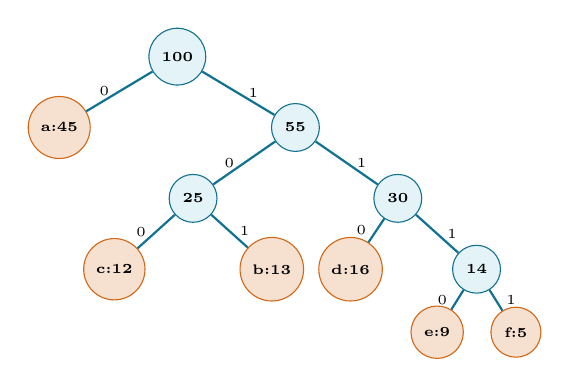
\begin{tikzpicture}[
        nd/.style={circle,draw=PrimaryMid,fill=PrimaryLight!40,
                   font=\bfseries\tiny,minimum size=0.55cm},
        leaf/.style={circle,draw=AccentOrange,fill=AccentOrange!20,
                     font=\bfseries\tiny,minimum size=0.55cm},
        arr/.style={draw=PrimaryMid,thick}
      ]
        \node[nd] (r) at (2.0,3.0) {100};
        \node[leaf] (a) at (0.5,2.1) {a:45};
        \node[nd]  (n55) at (3.5,2.1) {55};
        \node[nd]  (n25) at (2.2,1.2) {25};
        \node[nd]  (n30) at (4.8,1.2) {30};
        \node[leaf](c) at (1.2,0.3) {c:12};
        \node[leaf](b) at (3.2,0.3) {b:13};
        \node[leaf](d) at (4.2,0.3) {d:16};
        \node[nd]  (n14) at (5.8,0.3) {14};
        \node[leaf](e) at (5.3,-0.5) {e:9};
        \node[leaf](f) at (6.3,-0.5) {f:5};
        \draw[arr] (r)--node[left,font=\tiny]{0}(a);
        \draw[arr] (r)--node[right,font=\tiny]{1}(n55);
        \draw[arr] (n55)--node[left,font=\tiny]{0}(n25);
        \draw[arr] (n55)--node[right,font=\tiny]{1}(n30);
        \draw[arr] (n25)--node[left,font=\tiny]{0}(c);
        \draw[arr] (n25)--node[right,font=\tiny]{1}(b);
        \draw[arr] (n30)--node[left,font=\tiny]{0}(d);
        \draw[arr] (n30)--node[right,font=\tiny]{1}(n14);
        \draw[arr] (n14)--node[left,font=\tiny]{0}(e);
        \draw[arr] (n14)--node[right,font=\tiny]{1}(f);
      \end{tikzpicture}
  \end{columns}
\end{frame}

% ============================================================
\section{Dijkstra's Shortest Path}
% ============================================================

\begin{frame}[shrink=12]{Dijkstra's Algorithm}
  \begin{block}{Problem}
    Given a weighted graph with non-negative edge weights,
    find the \emph{shortest paths} from a single source vertex $s$
    to all other vertices.
  \end{block}
  \vspace{0.2em}
  \begin{columns}[T]
    \column{0.50\textwidth}
      \begin{block}{Algorithm}
        \begin{algorithmic}[1]
          \State $d[s] \gets 0$;\; $d[v] \gets \infty$ for $v \neq s$
          \State Priority queue $Q \gets$ all vertices
          \While{$Q$ not empty}
            \State $u \gets$ vertex in $Q$ with min $d[u]$
            \State remove $u$ from $Q$
            \For{each neighbour $v$ of $u$}
              \If{$d[u] + w(u,v) < d[v]$}
                \State $d[v] \gets d[u] + w(u,v)$
              \EndIf
            \EndFor
          \EndWhile
        \end{algorithmic}
      \end{block}
    \column{0.45\textwidth}
      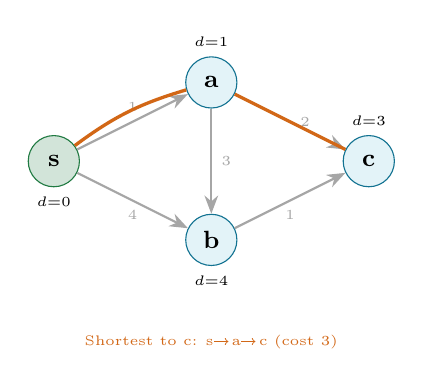
\begin{tikzpicture}[
        nd/.style={circle,draw=PrimaryMid,fill=PrimaryLight!40,
                   font=\bfseries\small,minimum size=0.65cm},
        vis/.style={circle,draw=SuccessGreen,fill=SuccessGreen!20,
                    font=\bfseries\small,minimum size=0.65cm},
        arr/.style={-{Stealth},gray!70,thick}
      ]
        \node[vis] (s) at (0,2) {s};
        \node[nd]  (a) at (2,3) {a};
        \node[nd]  (b) at (2,1) {b};
        \node[nd]  (c) at (4,2) {c};
        \draw[arr] (s)--node[above,font=\tiny]{1}(a);
        \draw[arr] (s)--node[below,font=\tiny]{4}(b);
        \draw[arr] (a)--node[right,font=\tiny]{2}(c);
        \draw[arr] (b)--node[below,font=\tiny]{1}(c);
        \draw[arr] (a)--node[right,font=\tiny]{3}(b);
        \node[font=\tiny,below] at (s.south) {$d{=}0$};
        \node[font=\tiny,above] at (a.north) {$d{=}1$};
        \node[font=\tiny,below] at (b.south) {$d{=}4$};
        \node[font=\tiny,above] at (c.north) {$d{=}3$};
        \draw[AccentOrange,very thick]
          (s)edge[bend left=10](a) (a)--(c);
        \node[font=\tiny,text=AccentOrange] at (2,-0.3)
          {Shortest to c: s→a→c (cost 3)};
      \end{tikzpicture}

      \textbf{Complexity:} $\mathcal{O}((|V|+|E|)\log|V|)$ with binary heap.
  \end{columns}
\end{frame}

% ============================================================
\section{Minimum Spanning Trees}
% ============================================================

\begin{frame}[shrink=12]{Minimum Spanning Tree — Problem}
  \begin{block}{Definition}
    A \keyword{spanning tree} of a connected graph $G=(V,E)$ is a
    sub-graph that is a tree containing all $|V|$ vertices.
    A \keyword{minimum spanning tree (MST)} has the minimum total
    edge weight among all spanning trees.
  \end{block}
  \vspace{0.4em}
  \begin{columns}[T]
    \column{0.50\textwidth}
      \textbf{Applications:}
      \begin{itemize}
        \item Network design (cable layout, pipelines)
        \item Cluster analysis in machine learning
        \item Circuit board design (VLSI)
        \item Approximation algorithms for TSP
      \end{itemize}
      \vspace{0.3em}
      \textbf{Two greedy algorithms:}
      \begin{enumerate}
        \item \keyword{Prim's algorithm} — grow one tree, add nearest vertex
        \item \keyword{Kruskal's algorithm} — add cheapest safe edge
      \end{enumerate}
    \column{0.45\textwidth}
      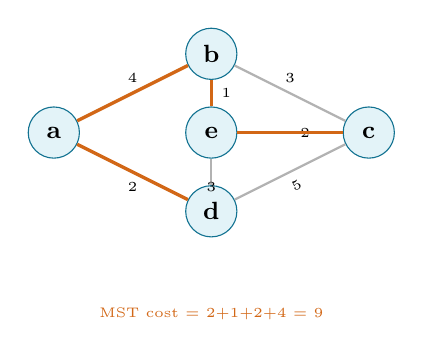
\begin{tikzpicture}[
        nd/.style={circle,draw=PrimaryMid,fill=PrimaryLight!40,
                   font=\bfseries\small,minimum size=0.65cm},
        mst/.style={draw=AccentOrange,very thick},
        reg/.style={draw=gray!60,thick}
      ]
        \node[nd] (a) at (0,2) {a};
        \node[nd] (b) at (2,3) {b};
        \node[nd] (c) at (4,2) {c};
        \node[nd] (d) at (2,1) {d};
        \node[nd] (e) at (2,2) {e};
        \draw[reg] (a)--(b) node[midway,above,font=\tiny]{4};
        \draw[reg] (a)--(d) node[midway,below,font=\tiny]{2};
        \draw[reg] (b)--(c) node[midway,above,font=\tiny]{3};
        \draw[reg] (b)--(e) node[midway,right,font=\tiny]{1};
        \draw[reg] (c)--(e) node[midway,right,font=\tiny]{2};
        \draw[reg] (d)--(e) node[midway,below,font=\tiny]{3};
        \draw[reg] (c)--(d) node[midway,below,font=\tiny,sloped]{5};
        % MST edges
        \draw[mst] (a)--(d);
        \draw[mst] (b)--(e);
        \draw[mst] (c)--(e);
        \draw[mst] (a)--(b);
        \node[font=\tiny,text=AccentOrange] at (2,-0.3)
          {MST cost = 2+1+2+4 = 9};
      \end{tikzpicture}
  \end{columns}
\end{frame}

\begin{frame}[shrink=12]{Prim's Algorithm}
  \begin{columns}[T]
    \column{0.50\textwidth}
      \textbf{Strategy:} Start with any vertex; repeatedly add the
      \emph{minimum-weight edge} connecting the MST so far to a vertex
      not yet in it.

      \vspace{0.3em}
      \begin{block}{Algorithm}
        \begin{algorithmic}[1]
          \State $T \gets \{v_0\}$, $E_T \gets \emptyset$
          \While{$|T| < n$}
            \State Find min-weight edge $(u,v)$ with
                   $u \in T$, $v \notin T$
            \State $T \gets T \cup \{v\}$;\;
                   $E_T \gets E_T \cup \{(u,v)\}$
          \EndWhile
          \State \Return $(T, E_T)$
        \end{algorithmic}
      \end{block}
    \column{0.45\textwidth}
      \begin{alertblock}{Complexity}
        With adjacency matrix: $\Theta(n^2)$\\
        With min-heap: $\mathcal{O}(|E|\log|V|)$
      \end{alertblock}
      \vspace{0.3em}
      \textbf{Why it is correct:} \emph{Cut property}:
      for any cut $(S, V\setminus S)$ of the graph, the minimum-weight
      edge crossing the cut is safe to add to the MST.
      (Proof by exchange argument.)

      \vspace{0.3em}
      \begin{exampleblock}{Related problem}
        Prim's algorithm is analogous to \emph{Dijkstra's}; the only
        difference is the priority key: distance vs.\ edge weight.
      \end{exampleblock}
  \end{columns}
\end{frame}

\begin{frame}[shrink=12]{Kruskal's Algorithm}
  \begin{columns}[T]
    \column{0.50\textwidth}
      \textbf{Strategy:} Sort all edges by weight; add an edge if it
      does not create a cycle (check with Union-Find).

      \vspace{0.3em}
      \begin{block}{Algorithm}
        \begin{algorithmic}[1]
          \State Sort edges $e_1\leq e_2\leq\cdots\leq e_{|E|}$
          \State Initialise Union-Find on $V$
          \State $E_T \gets \emptyset$
          \For{$i \gets 1$ \textbf{to} $|E|$}
            \If{$e_i = (u,v)$ and $\text{Find}(u) \neq \text{Find}(v)$}
              \State $E_T \gets E_T \cup \{e_i\}$
              \State $\text{Union}(u, v)$
            \EndIf
          \EndFor
          \State \Return $E_T$
        \end{algorithmic}
      \end{block}
    \column{0.45\textwidth}
      \begin{alertblock}{Complexity}
        Sorting: $\mathcal{O}(|E|\log|E|)$\\
        Union-Find: $\mathcal{O}(|E|\cdot\alpha(|V|))$ (near-linear)\\
        \textbf{Total:} $\mathcal{O}(|E|\log|E|)$
      \end{alertblock}
      \vspace{0.3em}
      \textbf{Prim's vs.\ Kruskal's:}
      \begin{tabular}{lll}
        & Prim & Kruskal \\
        \midrule
        Dense graphs & Better & Slower \\
        Sparse graphs & Equal & Better \\
        Data structure & Priority Q & Union-Find \\
      \end{tabular}
      \vspace{0.2em}
      Both produce an MST with weight $= \sum_{e\in E_T} w(e)$.
  \end{columns}
\end{frame}

% ============================================================
\section{Greedy vs.\ Dynamic Programming}
% ============================================================

\begin{frame}[shrink=12]{When to Use Which?}
  \begin{columns}[T]
    \column{0.55\textwidth}
      \begin{tabular}{lll}
        \toprule
        \textbf{Problem} & \textbf{Greedy} & \textbf{DP} \\
        \midrule
        Activity selection & \textcolor{SuccessGreen}{\checkmark} optimal & Yes \\
        Huffman coding & \textcolor{SuccessGreen}{\checkmark} optimal & Yes \\
        MST (Prim, Kruskal) & \textcolor{SuccessGreen}{\checkmark} optimal & N/A \\
        0-1 Knapsack & \alert{suboptimal} & \textcolor{SuccessGreen}{\checkmark} optimal \\
        Change-making (US) & \textcolor{SuccessGreen}{\checkmark} optimal & Yes \\
        Change-making (gen.) & \alert{suboptimal} & \textcolor{SuccessGreen}{\checkmark} optimal \\
        Shortest path (dag) & \textcolor{SuccessGreen}{\checkmark} optimal & Yes \\
        TSP & \alert{heuristic only} & exact (slow) \\
        \bottomrule
      \end{tabular}
    \column{0.40\textwidth}
      \begin{block}{Decision guide}
        \begin{enumerate}
          \item Does the problem have \emph{optimal substructure}?
          \begin{itemize}
            \item No → neither works directly
          \end{itemize}
          \item Does it have \emph{overlapping sub-problems}?
          \begin{itemize}
            \item Yes → likely DP
            \item No → likely D\&C
          \end{itemize}
          \item Does the \emph{greedy choice property} hold?
          \begin{itemize}
            \item Yes → greedy (faster)
            \item No → DP (always correct)
          \end{itemize}
        \end{enumerate}
      \end{block}
  \end{columns}
\end{frame}

% ── Chapter Summary ──────────────────────────────────────────
\begin{frame}[shrink=12]{Chapter 7 Summary}
  \begin{columns}[T]
    \column{0.55\textwidth}
      \textbf{Greedy algorithms studied:}
      \begin{tabular}{ll}
        \toprule
        Problem & Complexity \\
        \midrule
        Activity selection & $\mathcal{O}(n\log n)$ \\
        Huffman coding & $\mathcal{O}(n\log n)$ \\
        Dijkstra's SSSP & $\mathcal{O}((|V|{+}|E|)\log|V|)$ \\
        Prim's MST & $\mathcal{O}(|E|\log|V|)$ \\
        Kruskal's MST & $\mathcal{O}(|E|\log|E|)$ \\
        \bottomrule
      \end{tabular}
      \vspace{0.3em}
      \textbf{Key: prove correctness} using exchange argument or
      cut property before claiming a greedy algorithm is optimal.
    \column{0.40\textwidth}
      \begin{block}{Course Summary}
        You have now studied all major algorithm design paradigms:
        \begin{itemize}
          \item \keyword{Brute Force}
          \item \keyword{Decrease \& Conquer}
          \item \keyword{Divide \& Conquer}
          \item \keyword{Transform \& Conquer}
          \item \keyword{Dynamic Programming}
          \item \keyword{Greedy Algorithms}
        \end{itemize}
      \end{block}
      \begin{exampleblock}{Next steps}
        NP-completeness, approximation algorithms, and randomised
        algorithms are advanced topics that build on this foundation.
      \end{exampleblock}
  \end{columns}
\end{frame}

\end{document}
